%%%%%%%%%%%%%%%%%%%%% chapter.tex %%%%%%%%%%%%%%%%%%%%%%%%%%%%%%%%%
%
% sample chapter
%
% Use this file as a template for your own input.
%
%%%%%%%%%%%%%%%%%%%%%%%% Springer-Verlag %%%%%%%%%%%%%%%%%%%%%%%%%%
%\motto{Use the template \emph{chapter.tex} to style the various elements of your chapter content.}
\chapter{Example C: two sector economy}
\chaptermark{Example C}
\label{chap:two_sector} % Always give a unique label
% use \chaptermark{}
% to alter or adjust the chapter heading in the running head

\abstract*{[NEED TO ADD ABSTRACT HERE]}

%% \abstract{Each chapter should be preceded by an abstract (10--15 lines long) that summarizes the content. The abstract will appear \textit{online} at \url{www.SpringerLink.com} and be available with unrestricted access. This allows unregistered users to read the abstract as a teaser for the complete chapter. As a general rule the abstracts will not appear in the printed version of your book unless it is the style of your particular book or that of the series to which your book belongs.\newline\indent
%% Please use the 'starred' version of the new Springer \texttt{abstract} command for typesetting the text of the online abstracts (cf. source file of this chapter template \texttt{abstract}) and include them with the source files of your manuscript. Use the plain \texttt{abstract} command if the abstract is also to appear in the printed version of the book.}

%% Use the template \emph{chapter.tex} together with the Springer document class SVMono (monograph-type books) or SVMult (edited books) to style the various elements of your chapter content in the Springer layout.


We extend single-sector Example B to derive a matrix representation for the I-O method that can be generalized to any number of economic sectors. A two-sector economy consisting of an Energy sector (3) and a Goods and Services sector (4) is considered. Both the Earth (1) and Society (2) are also included. Resources are extracted from the Earth (1), and Society (2) provides the final demand for both the Goods and Services (4) and the Energy (3) sectors.

%%%%%%%%%% Example C %%%%%%%%%%
\section{First Law of Thermodynamics}
%%%%%%%%%%

The First Law of Thermodynamics requires that energy is conserved around each sector of the economy as well as around the Earth (1) and Society (2) as shown in Figure \ref{fig:direct_energy_flows_2}. 

\begin{figure}[h!]
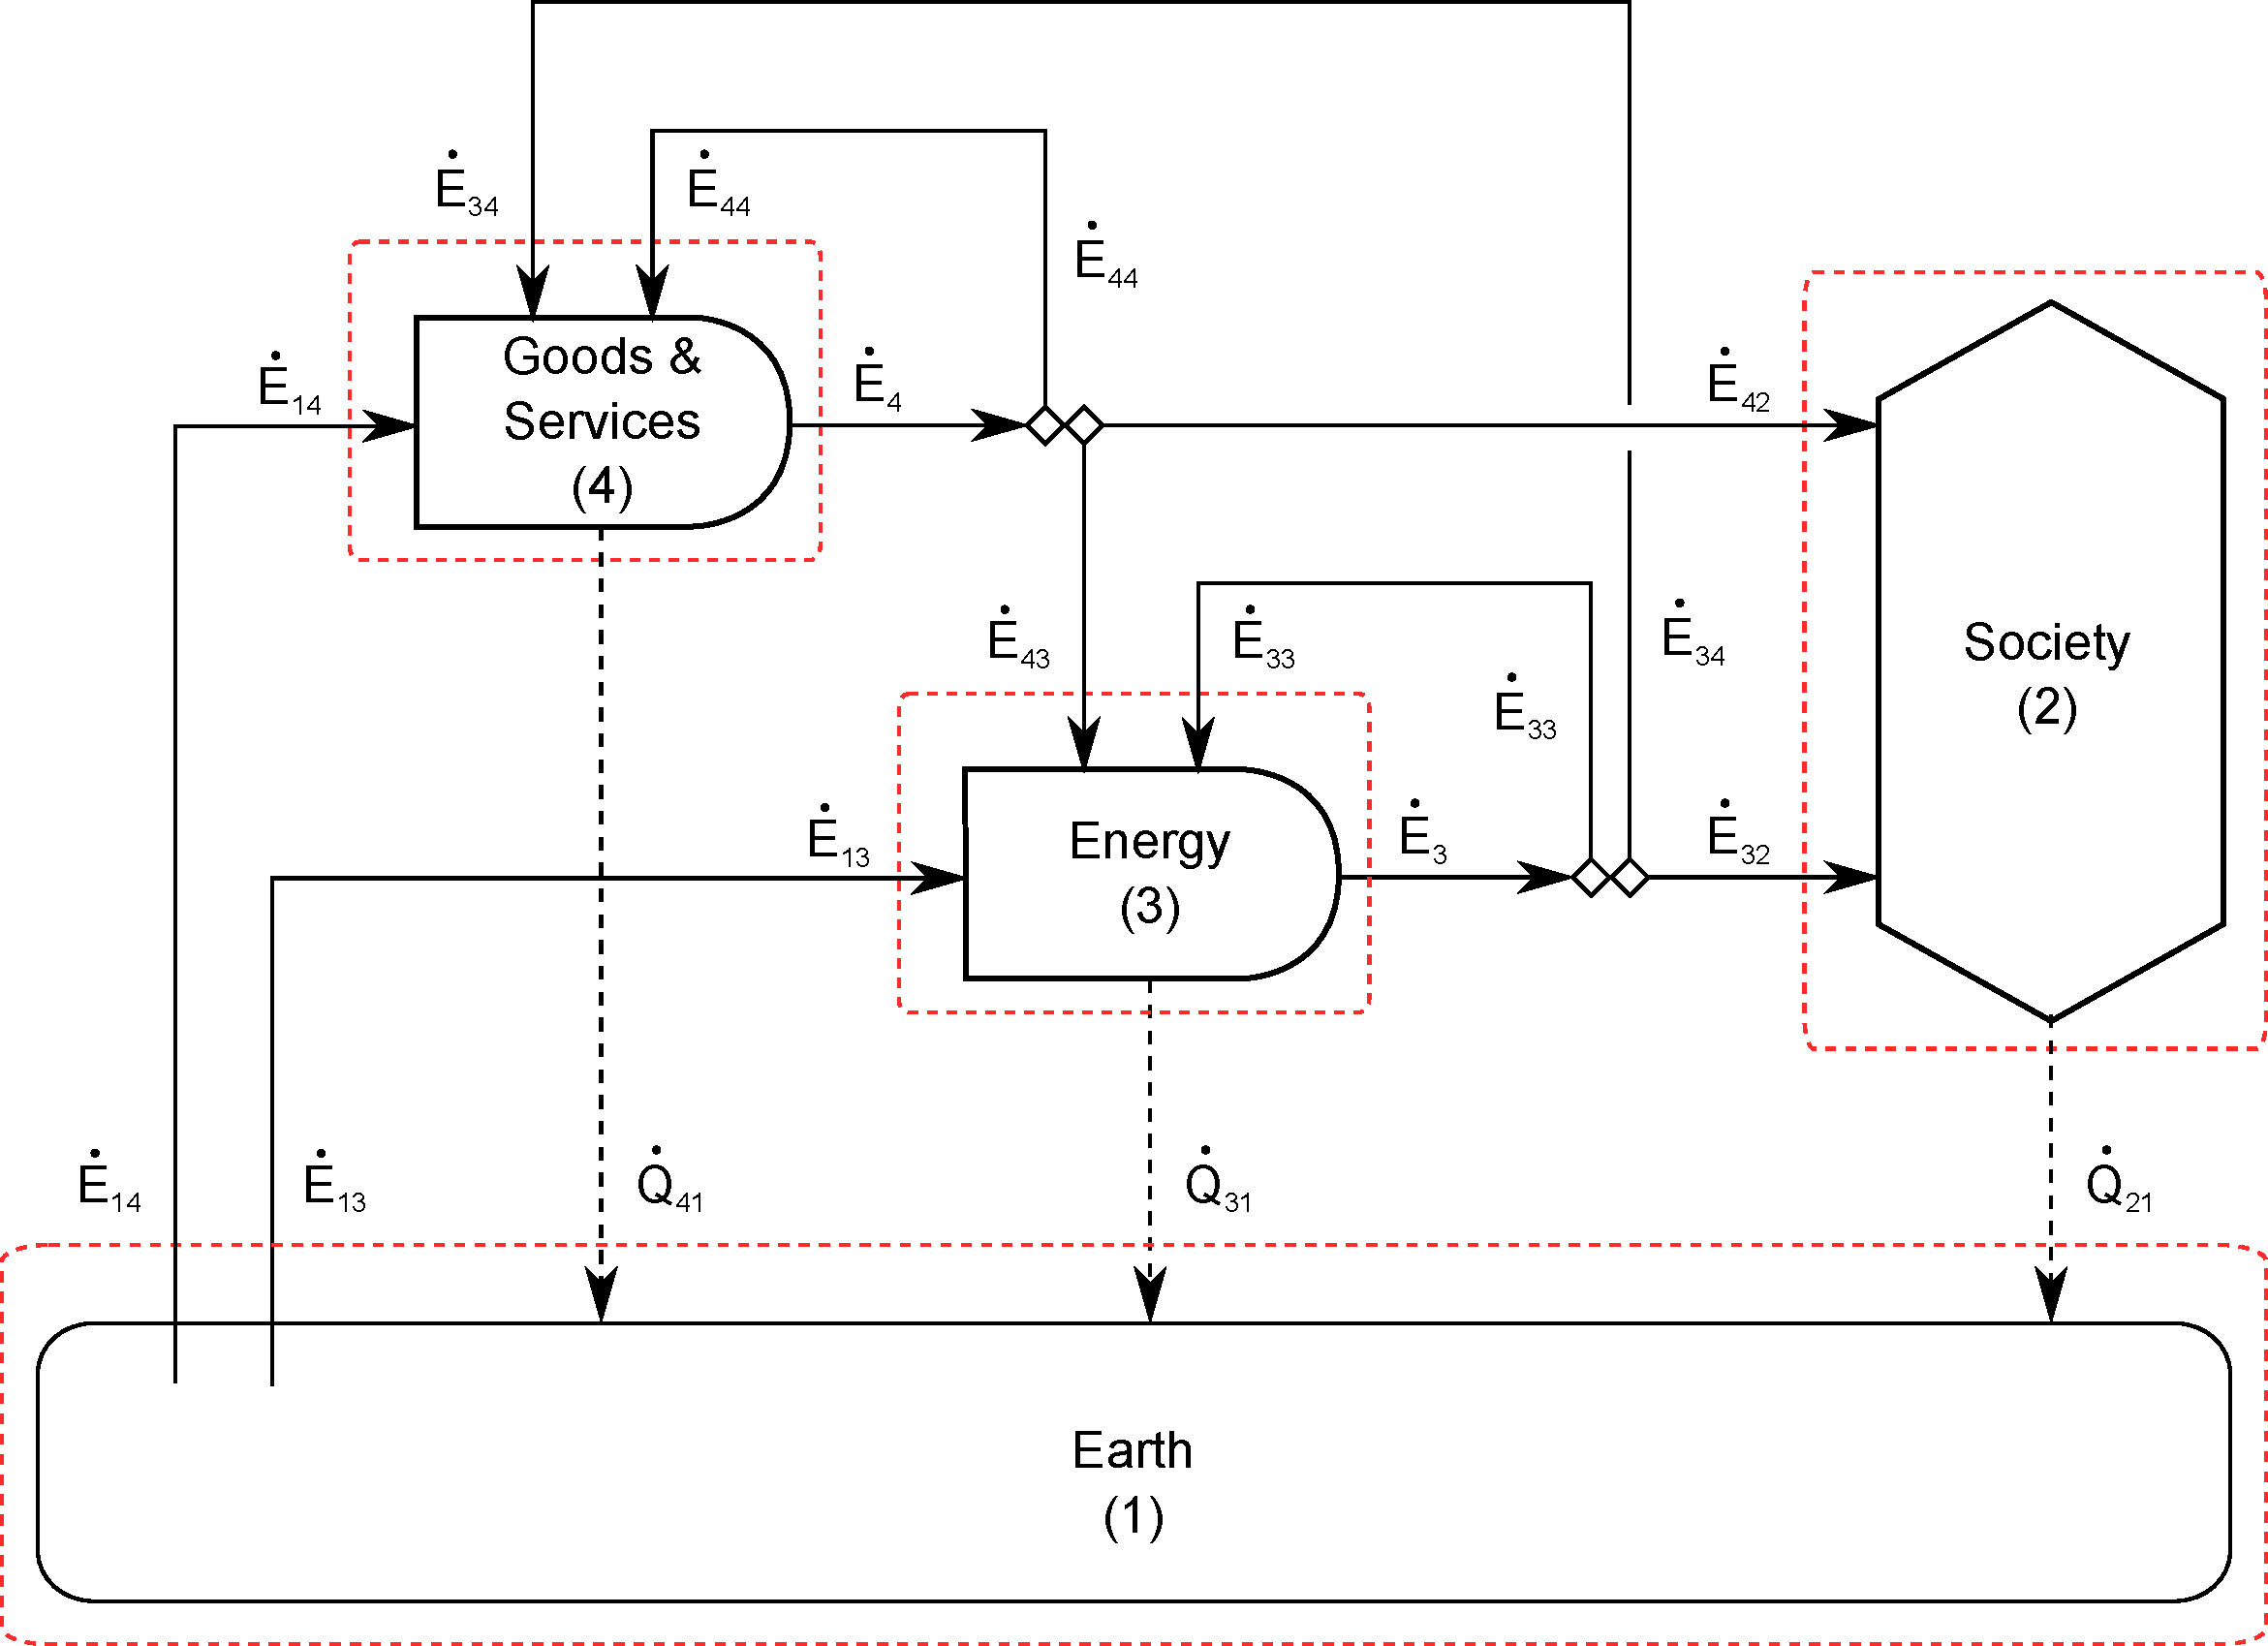
\includegraphics[width=1.0\linewidth]{Chapter_Example_C/images/I-O_three_sector_direct_energy.pdf}
\caption{Flows of direct energy ($\dot{E}$) and waste heat ($\dot{Q}$) in a two-sector economy.}
\label{fig:direct_energy_flows_2}
\end{figure}

In this economy, we assume that the purpose of the Goods and Services sector (4) is to produce goods and provide services, it provides no direct energy to society. The purpose of the Energy sector (3) is to make direct energy ($\dot{E}$) available to the economy and society in a useful form. Both direct energy ($\dot{E}$) (such as chemical potential energy in coal, oil, and electricity) and waste heat ($\dot{Q}$) are accounted by the First Law of Thermodynamics. The First Law around the Goods and Services sector (4) including, for now, the accumulation rate of direct energy in the sector $\left(\frac{\mathrm{d}E_{4}}{\mathrm{d}t}\right)$ yields

\begin{equation} \label{eq:C-CV_E_dot_4}
	\frac{\mathrm{d}E_{4}}{\mathrm{d}t} 	 =  \dot{E}_{14} + \dot{E}_{34} + \dot{E}_{44} - \dot{E}_4 - \dot{Q}_{41}.
\end{equation}

Note that we may simplify Equation \ref{eq:C-CV_E_dot_4} by realizing that $\dot{E}_{4} = \dot{E}_{4i} = 0$, because the goods and services sector is assumed to produce no flows of energy, and that $\dot{E}_{14} = 0$, since sector (4) receives no direct energy from the earth, except via the energy sector (3), hence:

\begin{equation} \label{eq:C-CV_E_dot_4_simp}
	\frac{\mathrm{d}E_{4}}{\mathrm{d}t} 	 =  \dot{E}_{34} - \dot{Q}_{41}.
\end{equation}

% [HOW DO WE WANT TO ACCOUNT FOR FOOD (i.e. ENERGY) OUTPUT FROM SECTOR (4) WHICH FLOWS INTO SECTOR (2) IN THIS FRAMEWORK? SIMILARLY, THERE ARE ENERGY FLOWS WHICH ARE USED INTERNALLY (E.G. FERTILIZERS, SO SHOULD WE HAVE $\dot{E}_{4}$ and $\dot{E}_{44}$ TERMS] 
% [ANOTHER CONCEPTUAL QUESTION IS WHETHER AN $\dot{E}_{24}$ TERM SHOULD BE INCLUDED. LABOR IS SUPPLIED FROM SOCIETY TO THE GOODS AND SERVICES SECTOR. LABOR IS A FORM OF DIRECT ENERGY, NO? --MKH]
% [FOOTNOTE ADDED TO DEAL WITH TWO COMMENTS ABOVE - MD]

%[I DECIDED TO INCLUDE THE $\dot{E_4}$ TERM IN THE ABOVE EQUATION. WE DON'T NEED AN $\dot{E}_{44}$ TERM. --MKH. I DON'T FOLLOW WHY WE DON'T NEED THE $\dot{E}_{44}$ TERM? - MD.]



The First Law of Thermodynamics around the Earth (1), Society (2), and the Energy sector (3) gives

\begin{equation} \label{eq:C-CV_E_dot_1}
	\frac{\mathrm{d}E_{1}}{\mathrm{d}t} 	 =  \dot{Q}_{21} + \dot{Q}_{31} + \dot{Q}_{41} - \dot{E}_{13} - \dot{E}_{14},
\end{equation}

\begin{equation} \label{eq:C-CV_E_dot_2}
	\frac{\mathrm{d}E_{2}}{\mathrm{d}t} 	 = \dot{E}_{32}  + \dot{E}_{42} - \dot{Q}_{21},
\end{equation}

\noindent and 

\begin{equation} \label{eq:C-CV_E_dot_3}
	\frac{\mathrm{d}E_{3}}{\mathrm{d}t} 	 = \dot{E}_{13} + \dot{E}_{33} + \dot{E}_{43} - \dot{E}_{3} - \dot{Q}_{31}.
\end{equation}

As in Examples A and B, we can set the accumulation of direct energy to zero.

\begin{equation} \label{eq:C-CV_E_dot_1_SS}
	0 =  \dot{Q}_{21} + \dot{Q}_{31} + \dot{Q}_{41} - \dot{E}_{13} - \dot{E}_{14}
\end{equation}

\begin{equation} \label{eq:C-CV_E_dot_2_SS}
	0  = \dot{E}_{32}  + \dot{E}_{42} - \dot{Q}_{21}
\end{equation}

\begin{equation} \label{eq:C-CV_E_dot_3_SS}
	0 = \dot{E}_{13} + \dot{E}_{33} + \dot{E}_{43} - \dot{E}_{3} - \dot{Q}_{31}
\end{equation}

\noindent and 

\begin{equation} \label{eq:C-CV_E_dot_4_SS}
	0 = \dot{E}_{14} + \dot{E}_{34} + \dot{E}_{44} - \dot{E}_4 - \dot{Q}_{41}
\end{equation}

%%%%%%%%%% Example C %%%%%%%%%%
\section{Total energy accounting}
%%%%%%%%%%

Again, we follow the I-O literature in assuming that total energy (i.e., the sum of direct energy and embodied energy) is conserved. Thus, we can draw a diagram similar to Figure \ref{fig:direct_energy_flows_2} for total energy flows.

\begin{figure}[h!]
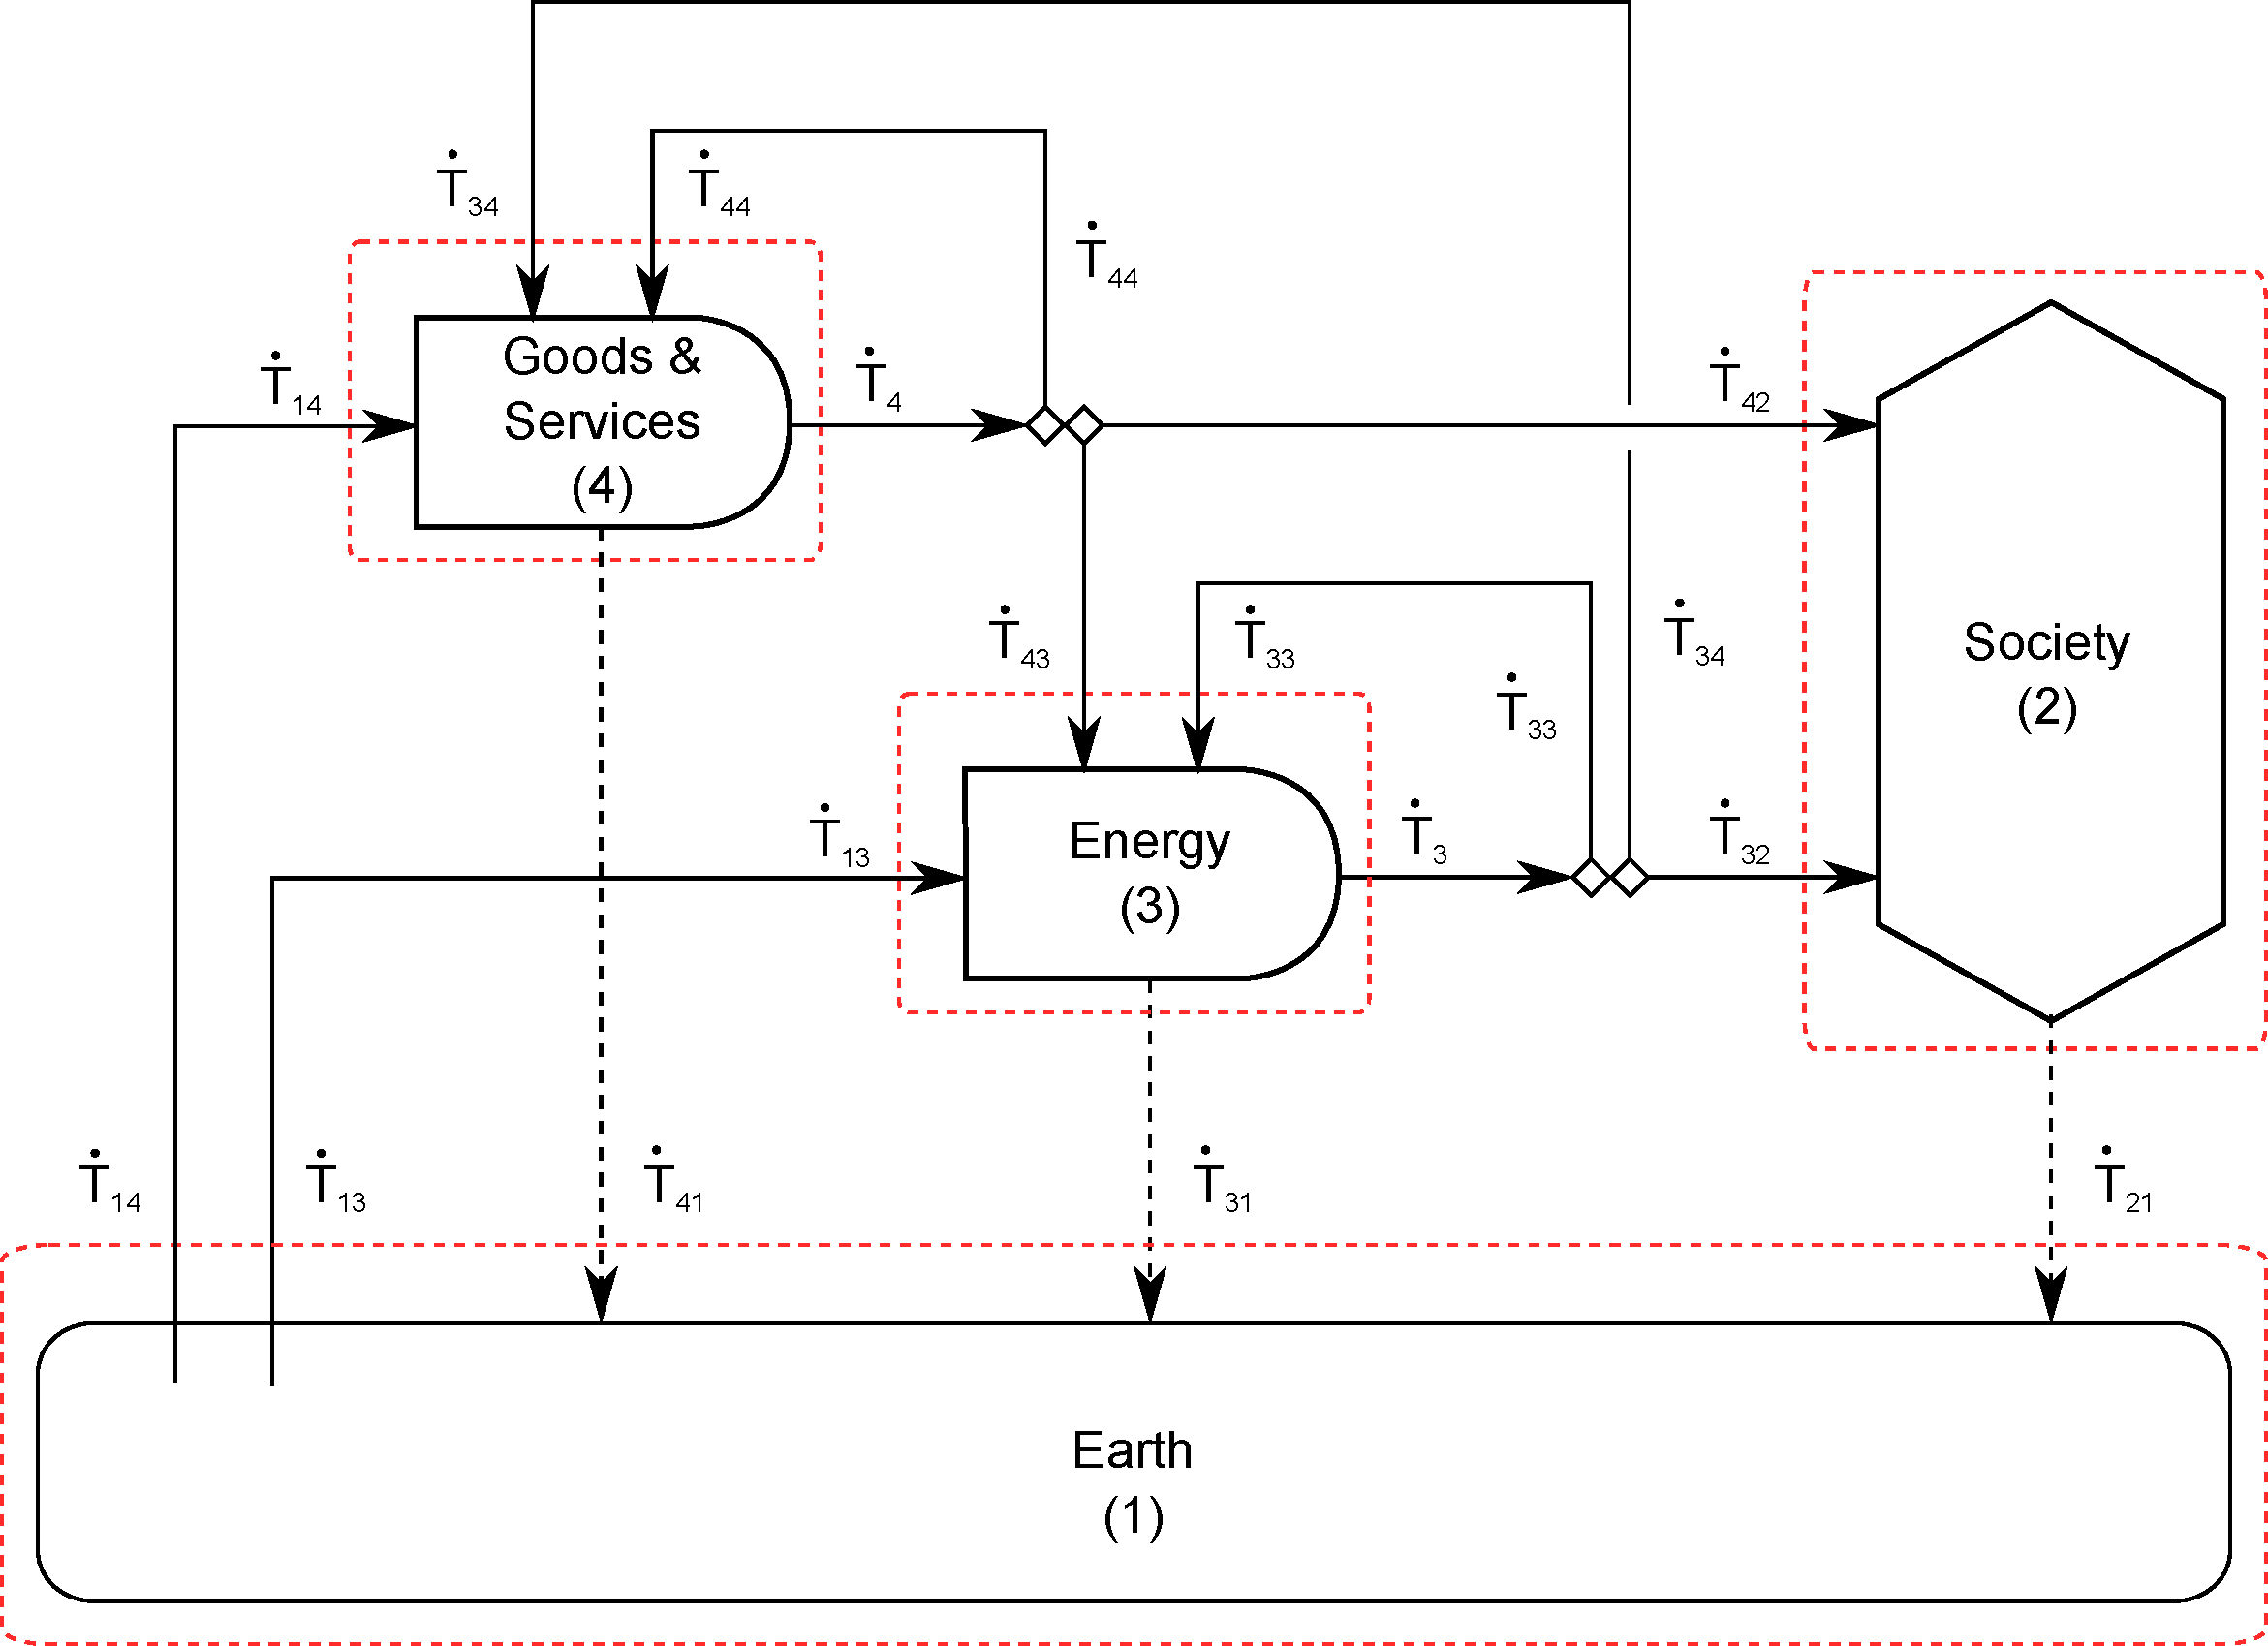
\includegraphics[width=1.0\linewidth]{Chapter_Example_C/images/I-O_three_sector_total_energy.pdf}
\caption{Flows of total energy ($\dot{T}$) in a two-sector economy.}
\label{fig:total_energy_flows_2S}
\end{figure}

Accounting for accumulation of total energy and using the assumption that total energy is conserved, we can write the following equations.

\begin{equation} \label{eq:C-CV_T_1}
	\frac{\mathrm{d}T_{1}}{\mathrm{d}t} 	 = \dot{T}_{21} + \dot{T}_{31} + \dot{T}_{41} - \dot{T}_{13} - \dot{T}_{14},
\end{equation}

\begin{equation} \label{eq:C-CV_T_2}
	\frac{\mathrm{d}T_{2}}{\mathrm{d}t} 	 = \dot{T}_{32} + \dot{T}_{42} - \dot{T}_{21},
\end{equation}

\begin{equation} \label{eq:C-CV_T_3}
	\frac{\mathrm{d}T_{3}}{\mathrm{d}t} 	 = \dot{T}_{13} + \dot{T}_{33} + \dot{T}_{43} - \dot{T}_{3} - \dot{T}_{31},
\end{equation}

\noindent and 

\begin{equation} \label{eq:C-CV_T_4}
	\frac{\mathrm{d}T_{4}}{\mathrm{d}t} 	 = \dot{T}_{14} + \dot{T}_{34} + \dot{T}_{44} - \dot{T}_{4} - \dot{T}_{41}.
\end{equation}

%%%%%%%%%% Example C %%%%%%%%%%
\section{Embodied energy accounting}
%%%%%%%%%%

Given that $\frac{\mathrm{d}E_{i}}{\mathrm{d}t} = 0$, we again note that $\frac{\mathrm{d}T_i}{\mathrm{d}t} = \frac{\mathrm{d}B_i}{\mathrm{d}t}$. Substituting $\dot{T} = \dot{E} + \dot{B}$ into the total energy accounting equations gives

\begin{equation} \label{eq:C-CV_dB_1}
	\frac{\mathrm{d}B_{1}}{\mathrm{d}t} 	 = \dot{E}_{21} + \dot{B}_{21} + \dot{E}_{31} + \dot{B}_{31} + \dot{E}_{41} + \dot{B}_{41} - \dot{E}_{13} - \dot{B}_{13} - \dot{E}_{14} - \dot{B}_{14},
\end{equation}

\begin{equation} \label{eq:C-CV_dB_2}
	\frac{\mathrm{d}B_{2}}{\mathrm{d}t} 	 = \dot{E}_{32} + \dot{B}_{32} + \dot{E}_{42} + \dot{B}_{42} - \dot{E}_{21} - \dot{B}_{21},
\end{equation}

\begin{equation} \label{eq:C-CV_dB_3}
	\frac{\mathrm{d}B_{3}}{\mathrm{d}t} 	 = \dot{E}_{13} + \dot{B}_{13} + \dot{E}_{33} + \dot{B}_{33} + \dot{E}_{43} + \dot{B}_{43} - \dot{E}_{3} - \dot{B}_{3} - \dot{E}_{31} - \dot{B}_{31},
\end{equation}

\noindent and 

\begin{equation} \label{eq:C-CV_dB_4}
	\frac{\mathrm{d}B_{4}}{\mathrm{d}t} 	 = \dot{E}_{14} + \dot{B}_{14} + \dot{E}_{34} + \dot{B}_{34} + \dot{E}_{44} + \dot{B}_{44} - \dot{E}_{4} - \dot{B}_{4} - \dot{E}_{41} - \dot{B}_{41}.
\end{equation}

Substituting the First Law of Thermodynamics (Equations \ref{eq:C-CV_E_dot_1_SS} through \ref{eq:C-CV_E_dot_4_SS}) into the total energy accounting equations (Equations \ref{eq:C-CV_dB_1} through \ref{eq:C-CV_dB_4}) gives embodied energy accounting equations for Example C.

\begin{equation} \label{eq:C-embodied_acct_1}
	\frac{\mathrm{d}B_{1}}{\mathrm{d}t} 	 = \dot{B}_{21} + \dot{B}_{31} + \dot{B}_{41} - \dot{B}_{13} - \dot{B}_{14} - \dot{Q}_{21} - \dot{Q}_{31} - \dot{Q}_{41}
\end{equation}

\begin{equation} \label{eq:C-embodied_acct_2}
	\frac{\mathrm{d}B_{2}}{\mathrm{d}t} 	 = \dot{B}_{32} + \dot{B}_{42} + \dot{Q}_{21} - \dot{B}_{21}
\end{equation}

\begin{equation} \label{eq:C-embodied_acct_3}
	\frac{\mathrm{d}B_{3}}{\mathrm{d}t} 	 = \dot{B}_{13} + \dot{B}_{33} + \dot{B}_{43} + \dot{Q}_{31} - \dot{B}_{3} - \dot{B}_{31}
\end{equation}

\begin{equation} \label{eq:C-embodied_acct_4}
	\frac{\mathrm{d}B_{4}}{\mathrm{d}t}	 = \dot{B}_{14} + \dot{B}_{34} + \dot{B}_{44} + \dot{Q}_{41} - \dot{B}_{4} - \dot{B}_{41}
\end{equation}

To verify the above derivation, we sum Equations \ref{eq:C-embodied_acct_1} through \ref{eq:C-embodied_acct_4} and use the following identities:

\begin{equation} \label{eq:C-B_sum_3_output}
	\dot{B}_3 = \dot{B}_{32} + \dot{B}_{33} + \dot{B}_{34}
\end{equation}

\noindent and

\begin{equation} \label{eq:C-B_sum_4_output}
	\dot{B}_4 = \dot{B}_{42} + \dot{B}_{43} + \dot{B}_{44};
\end{equation}

\noindent to obtain

\begin{equation} \label{eq:C-B_sums_to_zero}
	\frac{\mathrm{d}B_{1}}{\mathrm{d}t} + \frac{\mathrm{d}B_{2}}{\mathrm{d}t} + \frac{\mathrm{d}B_{3}}{\mathrm{d}t} + \frac{\mathrm{d}B_{4}}{\mathrm{d}t} = 0
\end{equation}

\noindent as expected. The total embodied energy content of the system (Earth (1), Society (2), Energy sector (3), and Goods and Services sector (4)) is constant with respect to time.


%%%%%%%%%% Example C %%%%%%%%%%
\section{Definition of embodied energy ($\dot{B}$)}\label{sec:embodied_energy}
%%%%%%%%%%

At this point we can develop a rigorous definition of embodied energy. To do so, we use the Goods and Services sector (4) from Example C. Direct energy accounting around the Goods and Services sector (Figure \ref{fig:direct_energy_flows_2}) yields

\begin{equation} \label{eq:CV_around_GS_sector_E_dot}
	\frac{\mathrm{d}E_{4}}{\mathrm{d}t} = \dot{E}_{14} + \dot{E}_{34} + \dot{E}_{44} - \dot{E}_{4} - \dot{Q}_{41},
\end{equation}

Total energy accounting around the Goods and Services sector (Figure \ref{fig:total_energy_flows_2S}) yields

\begin{equation} \label{eq:CV_around_GS_sector_T_dot}
	\frac{\mathrm{d}T_{4}}{\mathrm{d}t} = \dot{T}_{14} + \dot{T}_{34} + \dot{T}_{44} - \dot{T}_{4} + \dot{T}_{41},
\end{equation}

Solving the direct energy equation (Equation \ref{eq:CV_around_GS_sector_E_dot}) for the rate of direct energy input from the Energy sector (3) to the Goods and Services sector (4), namely $\dot{E}_{34}$, substituting into the total energy equation (Equation \ref{eq:CV_around_GS_sector_T_dot}), solving the result for $\dot{B}_{4}$, and assuming that no direct energy is wasted by the Goods and Services sector (4) to the Earth (1), i.e. $\dot{E}_{41} = 0$, yields

\begin{equation} \label{eq:embodied_output_GS}
	\dot{B}_{4} = \dot{B}_{14} + \dot{B}_{34} + \dot{B}_{44} + \dot{Q}_{41} - \frac{\mathrm{d}B_{4}}{\mathrm{d}t} - \dot{B}_{41}.
\end{equation}

Written generally, we obtain a formal definition for embodied energy output from an economic sector:

\begin{equation} \label{eq:embodied_def_1}
	\dot{B}_{j} \equiv \displaystyle\sum_{i} \dot{B}_{ij} - \frac{\mathrm{d}B_{j}}{\mathrm{d}t} - \dot{B}_{j1} + \dot{Q}_{j1}.
\end{equation}

Rearranging, we obtain

\begin{equation} \label{eq:embodied_def_2}
	\frac{\mathrm{d}B_{j}}{\mathrm{d}t} =  \displaystyle\sum_{i} \dot{B}_{ij} - \dot{B}_{j} - \dot{B}_{j1} + \dot{Q}_{j1}.
\end{equation}

In words, the rate of accumulation of embodied energy in a sector of the economy ($\frac{\mathrm{d}B_{j}}{\mathrm{d}t}$) is equal to the sum of the rates of input of embodied energy into the sector ($\displaystyle\sum_{i} \dot{B}_{ij}$) less the rate of useful output of embodied energy from the sector ($\dot{B}_{j}$) less  the rate of wasting embodied energy by the sector ($\dot{B}_{j1}$) \emph{plus} the rate of waste heat from the sector ($\dot{Q}_{j1}$). The first three terms on the right side of the equation are expected: accumulation is the difference between inflow and outflow rates. However, we see that the last term ($+\ \dot{Q}_{j1}$) in the above equations indicates that waste heat is \emph{additive} to both accumulation of embodied energy in a sector of the economy (Equation \ref{eq:embodied_def_2}) and outflow of embodied energy from a sector of the economy (Equation \ref{eq:embodied_def_1}). Furthermore, because the waste heat appears in the embodied energy output from a sector, waste heat accumulates along each step of a process such that the energy embodied in a finished product is the \emph{sum} of waste heats along a process path.


%%%%%%%%%% Example C %%%%%%%%%%
 \section{Depreciation}
%%%%%%%%%%

[SOMEWHERE WE NEED TO DISCUSS THE $\dot{S}_{i1}$ TERMS]

The terms $\dot{B}_{21}$,  $\dot{B}_{31}$, and $\dot{B}_{41}$ represent material depreciation (i.e., disposal) rates. As before, we can represent the embodied energy content of material depreciation as $\dot{B}_{i1} = \gamma_i B_i$ to obtain

\begin{equation} \label{eq:C-embodied_acct_1_depreciation}
	\frac{\mathrm{d}B_{1}}{\mathrm{d}t} 	 = \gamma_2 B_2 + \gamma_3 B_3 + \gamma_4 B_4 - \dot{B}_{13} - \dot{B}_{14} - \dot{Q}_{21} - \dot{Q}_{31} - \dot{Q}_{41}
\end{equation}

\begin{equation} \label{eq:C-embodied_acct_2_depreciation}
	\frac{\mathrm{d}B_{2}}{\mathrm{d}t} 	 = \dot{B}_{32} + \dot{B}_{42} + \dot{Q}_{21} - \gamma_2 B_2
\end{equation}

\begin{equation} \label{eq:C-embodied_acct_3_depreciation}
	\frac{\mathrm{d}B_{3}}{\mathrm{d}t} 	 = \dot{B}_{13} + \dot{B}_{33} + \dot{B}_{43} + \dot{Q}_{31} - \dot{B}_{3} - \gamma_3 B_3
\end{equation}

\begin{equation} \label{eq:C-embodied_acct_4_depreciation}
	\frac{\mathrm{d}B_{4}}{\mathrm{d}t}	 = \dot{B}_{14} + \dot{B}_{34} + \dot{B}_{44} + \dot{Q}_{41} - \dot{B}_{4} - \gamma_4 B_4
\end{equation}

%%%%%%%%%% Example C %%%%%%%%%%
%\section{Energy ratios}
%%%%%%%%%%%
%
%% [MIK: I MOVED THESE ENERGY RATIOS TO HERE FROM EARLIER, BECAUSE THEY NEED TO APPEAR AFTER WE DID THE TOTAL ENERGY ACCOUNTING FOR EXAMPLE C. YOU NEED TO REVIEW THIS SECTION IN LIGHT OF ALL OUR CHANGES. --MKH] 
%
%[THIS SECTION IS INTERESTING TO US, BUT MAY NOT BE GERMANE TO THE PAPER. IF THIS WERE TO BE A BOOK, I THINK WE SHOULD KEEP THIS SECTION IN. IF WE'RE NOW SHOOTING FOR A PAPER, WE CAN PROBABLY LEAVE THIS SECTION OUT. WE SHOULD AT LEAST REFERENCE THE LITERATURE HERE. OR, WE SHOULD MAKE USE OF THESE RATIOS. FOR EXAMPLE, IF WE WANT TO TALK ABOUT DECLINING RESOURCE QUALITY IN TERMS OF $EROI$ OR $GER$, WE SHOULD DO SO. WE SHOULD THEN SUBSTITUTE $GER$ INTO THE DERIVED EQUATIONS AND SHOW HOW A CHANGE IN $GER$ AFFECTS ENERGY FLOWS THROUGH THE ECONOMY.  --MKH]
%
%Several important energy ratios can be observed in Figure \ref{fig:direct_energy_flows_2}. [REFERENCE OTHER PAPERS FOR NOMENCLATURE? --MKH] The Gross Energy Ratio ($GER$) is defined as: 
%
%\begin{equation} \label{eq:C-GER_def}
%	GER_{\beta} \equiv \frac{\dot{E}_{3}}{\dot{E}_{33}}.
%\end{equation}
%
%\noindent The Net Energy Ratio ($NER$) is defined as [SHOULD THE NUMERATOR FOR $NER_\beta$ BE $\dot{E}_{32} + \dot{E}_{34}$? --MKH]
%
%[MIK SHOULD CHECK THE NEXT TWO EQUATIONS. ARE THEY CORRECT? --MKH]
%
%\begin{equation} \label{eq:NER_beta_def}
%	NER_{\beta} \equiv \frac{\dot{E}_{32}}{\dot{E}_{33}} = GER - 1.
%\end{equation}
%
%%[THESE DEFINITIONS ARE EQUIVALENT TO $\beta$ BOUNDARY DEFINED IN BRANDT AND DALE (2011). WE CAN DEFINE EXTERNAL ENERGY RATIO BY ACCOUNTING FOR TOTAL ENERGY FLOWS AS BELOW]
%
%[CAN WE SIMPLIFY THESE? FOR EXAMPLE, $\dot{E}_{43} = 0$, SO THE DENOMINATOR CAN BE SIMPLIFIED TO $\dot{B}_{43}$ --MKH]
%
%\begin{equation} \label{eq:C-GER_delta_def}
%	GER_{\delta} \equiv \frac{\dot{E}_{3}}{\dot{T}_{33} + \dot{T}_{43}};
%\end{equation}
%
%[THIS EQUATION DOESN'T LOOK RIGHT. IT IS SAME AS THE PREVIOUS EQUATION $GER - 1$, BUT HAS A DIFFERENT DENOMINATOR. MIK SHOULD CHECK. --MKH]
%\begin{equation} \label{eq:C-NER_delta_def}
%	NER_{\beta} \equiv \frac{\dot{E}_{32} + \dot{E}_{34}}{\dot{T}_{33} + \dot{T}_{43}} = GER - 1;
%\end{equation}
%
%We may also define a Gross External Energy Ratio (GEER) and Net External Energy Ratio (NEER), which account only for inputs from other sectors in the denominator:
%
%\begin{equation} \label{eq:C-GEER_delta_def}
%	GEER_{\delta} \equiv \frac{\dot{E}_{3}}{\dot{T}_{43}},
%\end{equation}
%
%and
%
%\begin{equation} \label{eq:C-NEER_delta_def}
%	NEER_{\beta} \equiv \frac{\dot{E}_{32}}{\dot{T}_{43}}.
%\end{equation}

%%%%%%%%%% Example C %%%%%%%%%%
\section{Final demand}
%%%%%%%%%%

Society's demand vector for total energy, $\dot{T}$, can be written as 

\begin{equation} \label{eq:demand_vector_T_dot}
	\vec{Y}_{\dot{T}} = 	\begin{Bmatrix} 	\dot{T}_{32}	\\
																\dot{T}_{42}	\\
									\end{Bmatrix}.
\end{equation}

\noindent In terms of total energy, the ultimate demand ($Y_{\dot{T}}$) is given by 

\begin{equation} \label{eq:final_demand_T_sum}
	Y_{\dot{T}} = 	\sum_{i=3}^{N} \dot{T}_{i2} = \dot{T}_{32} + \dot{B}_{42}.
\end{equation}

\noindent after realizing that $\dot{E}_{42} = 0$. 

[IS THE FOLLOWING PARAGRAPH IN THE RIGHT PLACE?]

We acknowledge that there are examples in the real economy which run counter to this model, where output from non-energy sectors are valued for their energetic content, one example being agriculture.  ``Direct'' energy inputs also flow in the opposite direction in the form of labor, which we also neglect. This will serve to introduce errors which will be small for industrial economies and larger for less industrial societies. To illustrate this we may compare the United States with India. To feed an adult requires around 2000 kcal/day $\approx$ 3 GJ/yr. To feed the whole $\sim$300 million population of the States requires around 1$\times 10^{18}$J (1 EJ) which is around 1\% of the roughly 100 EJ of primary energy supply. The US labor force currently stands at around 240 million. Given that a human can supply around 100 W of power and assuming an 8 hour work day, the US labor force will supply 70 TWh/yr $\approx$ 0.25 EJ. For India, the energy to food to feed 1.25 billion people is nearly 4 EJ which is around 15\% of the $\sim$25 EJ of primary energy consumed. Assuming that the labor force makes up 500 million people working at 12 hours per day, the energy supplied by labor is around 0.8 EJ or around 3\% of the total primary energy. As such, we can see that food energy accounts for around 1\% of primary energy in the US and around 15\% in India. Similarly, the labor inputs account for around 0.25\% in the US and around 3\% in India. The implication of including or omitting these flows is different in each case. Our assumptions introduce small errors for industrial societies where most of the world's energy is consumed.

Using $\dot{T}_{32} = \dot{E}_{32} + \dot{B}_{32}$ and rearranging Equation \ref{eq:final_demand_T_sum} gives

\begin{equation} \label{eq:rearranged_final_demand_T_sum}
	\dot{B}_{32} + \dot{B}_{42} = Y_{\dot{T}} - \dot{E}_{32}.
\end{equation}

\noindent Substituting Equation \ref{eq:rearranged_final_demand_T_sum} into Equation \ref{eq:C-embodied_acct_2_depreciation} yields

\begin{equation} \label{eq:intermediate_T_sum_dB2_dt}
	\frac{\mathrm{d}B_2}{\mathrm{d}t} = Y_{\dot{T}} - \dot{E}_{32} + \dot{Q}_{21} - \gamma_2 B_2.
\end{equation}

Substituting Equation \ref{eq:C-CV_E_dot_2_SS} into Eqaution \ref{eq:intermediate_T_sum_dB2_dt} and realizing that $\dot{E}_{42} = 0$ because direct energy is supplied to society by the energy sector only, we obtain 

\begin{equation} \label{eq:compare_demand_and_accumulation}
	\frac{\mathrm{d}B_{2}}{\mathrm{d}t} = Y_{\dot{T}} - \gamma_{2}B_{2},
\end{equation}

[IT WOULD BE GOOD TO FIND SOME VERY ROUGH DATA FOR THIS VALUE, E.G. WHAT IS THE AVERAGE LIFETIME OF MANUFACTURED GOODS - INCLUDING PACKAGING AND NON-CONSUMER GOODS. WHAT IS THE BALANCE OF NON-DURABLE VS. DURABLE GOODS? WHAT PROPORTION OF GOODS (E.G. FOOD) IS WASTED BEFORE EVER BEING CONSUMED?]

[I AGREE. HOW? --MKH]

\noindent indicating that the final demand vector for total energy ($Y_{\dot{T}}$) and the accumulation rate of energy in society $\left(\frac{\mathrm{d}B_{2}}{\mathrm{d}t}\right)$ differ by the rate of disposal from society ($\gamma_{2}B_{2}$). We note that as total embodied energy in society ($B_{2}$) becomes increasingly large, we need an ever-increasing rate of energy supplied to the society ($Y_{\dot{T}}$) to maintain positive growth $\left(\frac{\mathrm{d}B_{2}}{\mathrm{d}t}\right)$. [MAIN POINT THAT MUST BE DISCUSSED IN FURTHER DETAIL LATER, PARTICULARLY IN RELATION TO INCREASING GDP NOT NECESSARILY SIGNALING INCREASING ACCUMULATION OR GROWTH.]

%[WE NEVER USE THE FINAL PARAGRAPHS OF THIS SECTION. I PROPOSE THAT WE DELETE THEM. --MKH]
%
%A control volume around the economy gives
%
%\begin{equation} \label{eq:CV_around_economy_B_dot}
%	Y_{\dot{B}} = \sum_{j=1}^{N} \dot{E}_{1j} - \sum_{i=1}^{N} \dot{B}_{i1} - \dot{Q}_{21},
%\end{equation}
%
%[I HAVE ADDED $\dot{Q}_{21}$ TERM HERE, AS THERE IS DEFINITELY WASTE HEAT FROM CONSUMPTION OF FINAL ENERGY $Y_{\dot{B}}$ THAT IS NOT EMBODIED IN GOOD OR SERVICE, E.G. THE ELECTRICITY I USE TO COOK MY DINNER, OR WATCH TV]
%
%\noindent illustrating that final demand to society ($Y_{\dot{B}}$) can be considered the ultimate energy sink in the absence of depreciation in the economy.
%
%It is also interesting to note that 
%
%\begin{equation} \label{eq:flow_more_than_demand}
%	\sum_{i=1}^{N} \dot{T}_{i} > Y_{\dot{T}},
%\end{equation}
%
%\noindent which is a consequence of the self-demand of sectors within the economy.

%%%%%%%%%% Example C %%%%%%%%%%
\section{Flows of Value ($\dot{X}$)}
%%%%%%%%%%

The following figure shows value flows ($\dot{X}$) in the two-sector economy.

\begin{figure}[h!]
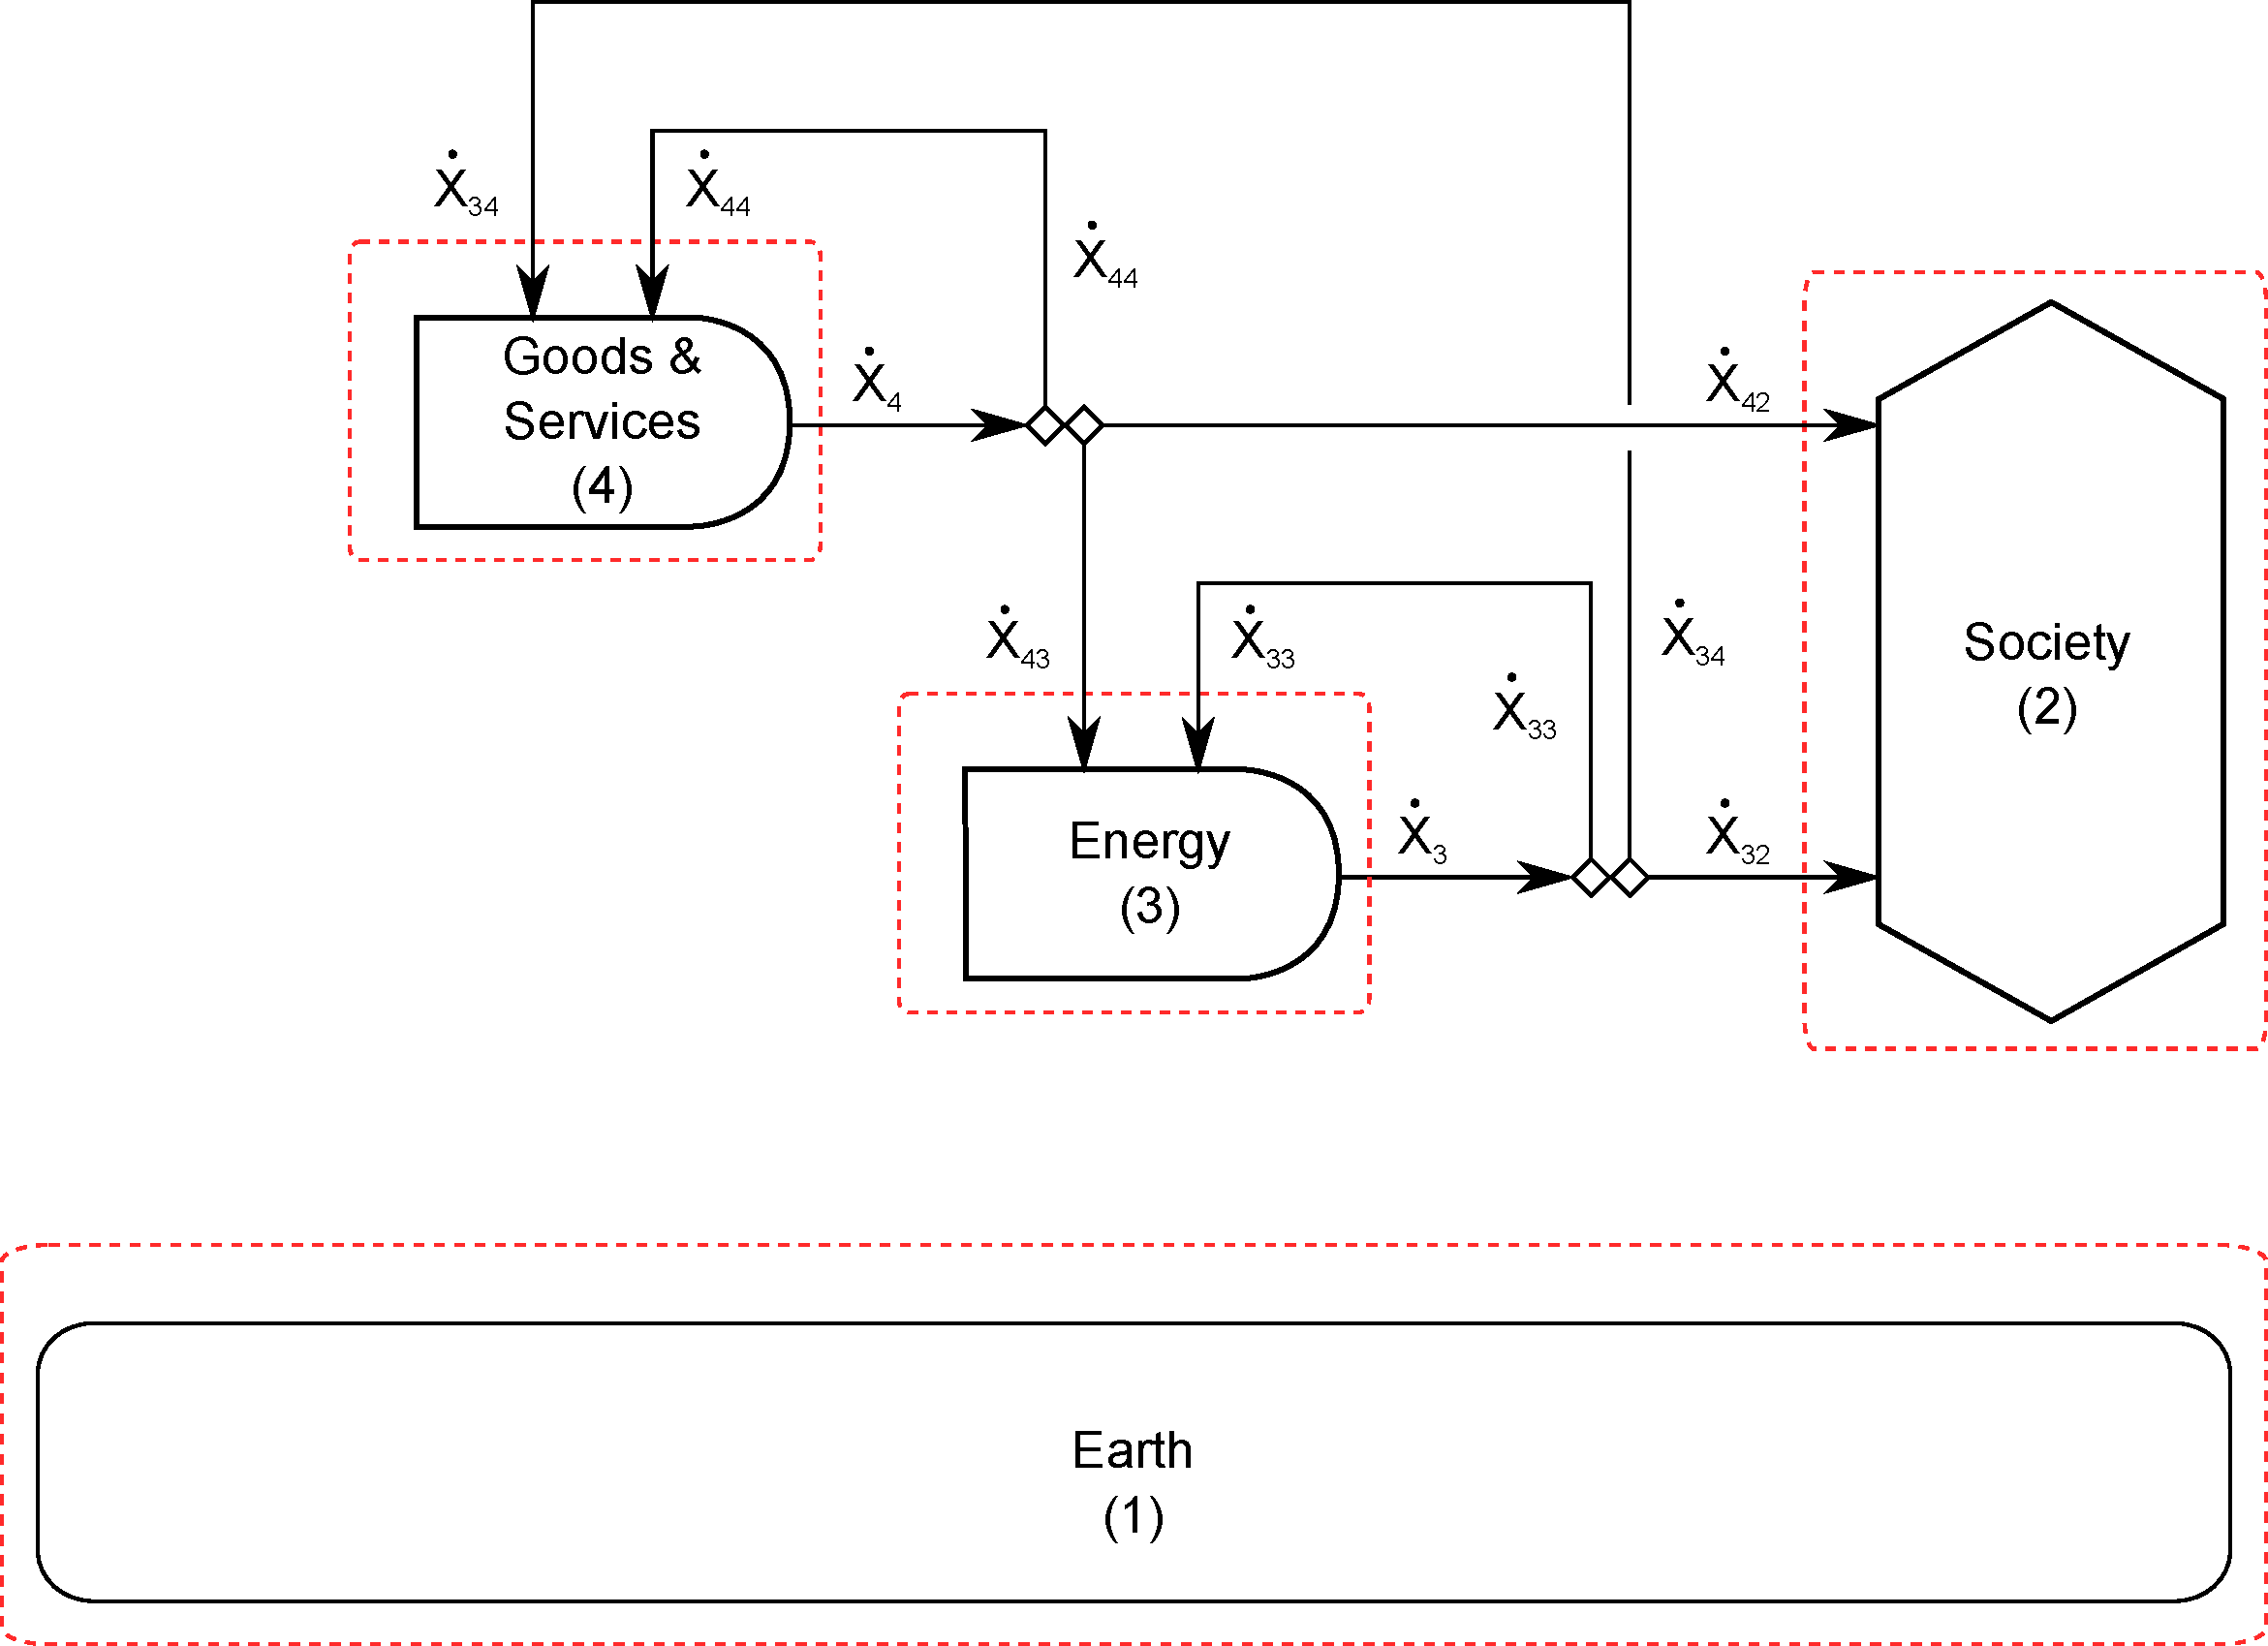
\includegraphics[width=1.0\linewidth]{Chapter_Example_C/images/I-O_three_sector_value.pdf}
\caption{Flows of economic value ($\dot{X}$) in a two-sector economy.}
\label{fig:economic_value_flows_2}
\end{figure}

Realizing that the valuable output from energy sectors is direct energy, $\dot{X}_{3} = \dot{E}_{3}$ and $\dot{X}_{3j} = \dot{E}_{3j}$. Thus, outputs from energy sectors are given in energy units (joules or BTUs). 

%With reference to Equations \ref{eq:GER_def_ch_5} and \ref{eq:NER_def_ch_5}, we can express the Gross Energy Ratio ($GER$) and Net Energy Ratio ($NER$) as
%
%\begin{equation} \label{eq:GER_in_terms_of_a_2}
%	GER_{\gamma} = \frac{\dot{E}_{3}}{\dot{E}_{33}} = \frac{\dot{X}_{3}}{\dot{X}_{33}} = \frac{1}{a_{33}},
%\end{equation}
%
%\noindent and
%
%\begin{equation} \label{eq:NER_in_terms_of_a_2}
%	NER = GER - 1 = \frac{1}{a_{33}} - 1.
%\end{equation}
%
%[DO WE NEED THESE NEXT TWO EQUATIONS? DO WE USE THEM ANYWHERE? THEY MIGHT BE HELPFUL FOR A GDP DISCUSSION, BUT WE HAVEN'T INCLUDED THAT DISCUSSION YET. --MKH]

Written in terms of value flows, the ultimate demand vector ($\vec{Y}$) is given by

\begin{equation} \label{eq:demand_vector_B_dot}
	\vec{Y}_{\dot{X}} = 	\begin{Bmatrix} 	\dot{X}_{32}	\\
																\dot{X}_{42}	\\
									\end{Bmatrix},
\end{equation}

\noindent and the total value demand from society ($Y$) is 

\begin{equation} \label{eq:total_value_demand}
	Y_{\dot{X}} = \sum_{i=1}^{N} \dot{X}_{i2} = \dot{X}_{32} + \dot{X}_{42}.
	\end{equation}


%%%%%%%%%% Example C %%%%%%%%%%
\section{Matrix Formulation}
%%%%%%%%%%

We can use Equations \ref{eq:epsilon_output_def} through \ref{eq:epsilon_equiv_1} to rewrite Equations \ref{eq:C-CV_B_1_depreciation} and \ref{eq:C-CV_B_2_depreciation} as

\begin{equation} \label{eq:CV_B_3_with_eps}
	\dot{X}_{33}\varepsilon_{3} + \dot{X}_{43}\varepsilon_{4} + \dot{E}_{13} - \frac{\mathrm{d}B_{3}}{\mathrm{d}t} - \gamma_{3}B_{3} = \dot{X}_{3}\varepsilon_{3}
\end{equation}

\noindent and 

\begin{equation} \label{eq:CV_B_4_with_eps}
	\dot{X}_{34}\varepsilon_{3} + \dot{X}_{44}\varepsilon_{4} + \dot{E}_{14} - \frac{\mathrm{d}B_{4}}{\mathrm{d}t} - \gamma_{4}B_{4} = \dot{X}_{4}\varepsilon_{4}.
\end{equation}

We can rewrite Equations \ref{eq:CV_B_3_with_eps} and \ref{eq:CV_B_4_with_eps} in matrix notation with the following definitions:

\begin{equation} \label{eq:eps_vec_def}
	\vec{\varepsilon} =		\begin{Bmatrix} 	\varepsilon_{3}	\\
																\varepsilon_{4}	\\
									\end{Bmatrix},
\end{equation}

\begin{equation} \label{eq:E_vec_def}
	\vec{E} =		\begin{Bmatrix} 	\dot{E}_{13}	\\
													\dot{E}_{14}\\
						\end{Bmatrix},
\end{equation}

\begin{equation} \label{eq:dBdt_vec_def}
	\frac{\mathrm{d}\vec{B}}{\mathrm{d}t} =	\begin{Bmatrix}	\frac{\mathrm{d}B_{3}}{\mathrm{d}t}	\\
																									\frac{\mathrm{d}B_{4}}{\mathrm{d}t}\\
																		\end{Bmatrix},
\end{equation}

\begin{equation} \label{eq:B_vec_def}
	\vec{B} =			\begin{Bmatrix}	B_{3}\\
														B_{4}\\
							\end{Bmatrix},
\end{equation}

\begin{equation} \label{eq:A_matrix_def}
	\vec{A} =	\begin{bmatrix} 	a_{33} & a_{34}	\\
												a_{43} & a_{44}	\\
					\end{bmatrix},
\end{equation}

\begin{equation} \label{eq:X_t_matrix_def}
	\vec{X}_{t} =		\begin{bmatrix} 	\dot{X}_{33}		&	\dot{X}_{34}	\\
														\dot{X}_{43}		&	\dot{X}_{44}\\
							\end{bmatrix},
\end{equation}

\begin{equation} \label{eq:X_hat_matrix_def}
	\hat{\vec{X}} = \delta_{ij}\dot{X}_{j} = \begin{bmatrix} 	\dot{X}_{33}		&	0					\\
																								0					&	\dot{X}_{44}	\\
																							\end{bmatrix},
\end{equation}

\begin{equation} \label{eq:B_hat_matrix_def}
	\hat{\vec{\gamma}} = \delta_{ij}\gamma_{j},
\end{equation}

[CAN WE MAKE THIS EQUATION EXPLICIT]

\noindent and

\begin{equation}\label{eq:k_delta}
	\delta_{ij} = \begin{cases}	1 	& 	\text{if  } i = j		\\
												0	&	\text{if  } i \neq j	\\
						\end{cases},
\end{equation}

\noindent such that:

\begin{equation} \label{eq:matrix_leontief}
	\vec{X}_{t}^{\mathrm{T}}\vec{\varepsilon} + \vec{E} - \left(\frac{\mathrm{d}\vec{B}}{\mathrm{d}t} + \hat{\vec{\gamma}}\vec{B}\right) = \hat{\vec{X}}\vec{\varepsilon}.
\end{equation}

Additional relationships that will be helpful later include (derived in Appendix):

\begin{equation} \label{eq:Xhat_X_and_A}
	\hat{\vec{X}}^{-1}\vec{X}_{t} = \vec{A}^{\mathrm{T}},
\end{equation}

\begin{equation} \label{eq:Xdifference1}
	\vec{X}_{t}^{\mathrm{T}} - \hat{\vec{X}} = \hat{\vec{X}}(\vec{A}^{\mathrm{T}} - \vec{I}),
\end{equation}

\begin{equation} \label{eq:Xdifference2}
	\hat{\vec{X}} - \vec{X}_{t}^{\mathrm{T}} = \hat{\vec{X}}(\vec{I} - \vec{A}^{\mathrm{T}}),
\end{equation}

\noindent and

\begin{equation} \label{eq:Xdifference2_inverse}
	\left(\hat{\vec{X}} - \vec{X}_{t}^{\mathrm{T}}\right)^{-1} = (\vec{I} - \vec{A}^{\mathrm{T}})^{-1}\hat{\vec{X}}^{-1}.
\end{equation}


%%%%%%%%%% Example C %%%%%%%%%%
\section{Estimating $\vec{\varepsilon}$ and $\frac{\mathrm{d}\vec{B}}{\mathrm{d}t}$}
%%%%%%%%%%

With Equation \ref{eq:matrix_leontief}, we can solve for either the energy accumulation vector ($\vec{\frac{\mathrm{d}B}{\mathrm{d}t}}$) or the energy intensity vector ($\vec{\varepsilon}$), but not both. 

Solving for the accumulation vector gives

\begin{equation} \label{eq:dB_dt_leontief}
	\frac{\mathrm{d}\vec{B}}{\mathrm{d}t} = (\vec{X}_{t}^{\mathrm{T}} - \hat{\vec{X}})\vec{\varepsilon} + \vec{E} - \hat{\vec{\gamma}}\vec{B}.
\end{equation}

\noindent Finally, we can substutute Equation \ref{eq:Xdifference1} which gives

\begin{equation} \label{eq:dB_dt_leontief_with_A}
	\frac{\mathrm{d}\vec{B}}{\mathrm{d}t} = \hat{\vec{X}} (\vec{A}^{\mathrm{T}} - \vec{I}) \vec{\varepsilon} + \vec{E} - \hat{\vec{\gamma}}\vec{B},
\end{equation}

\noindent which allows estimation of the embodied energy accumulation in economic sectors $\left(\frac{\mathrm{d}\vec{B}}{\mathrm{d}t}\right)$ knowing only sector outputs ($\hat{\vec{X}}$), sector input-output ratios ($\vec{A}$), sector energy intensities ($\vec{\varepsilon}$), energy input to the economy ($\vec{E}$), and sector physical depreciation rates ($\hat{\vec{\gamma}}\vec{b}$). In theory, the transaction matrix ($\vec{X}_{t}$) is not required if the input-ouput ratios ($\vec{A}$) are known, though in reality, knowledge of input-output ratios would be derived from the transaction matrix $\vec{X}_{t}$ .

Solving for the energy intensity vector gives

\begin{equation} \label{eq:epsilon_leontief}
	\vec{\varepsilon} = (\hat{\vec{X}} - \vec{X}_{t}^{\mathrm{T}})^{-1}\left[\vec{E} - \left(\frac{\mathrm{d}\vec{B}}{\mathrm{d}t} + \hat{\vec{\gamma}}\vec{B}\right)\right].
\end{equation}

\noindent Substituting Equation \ref{eq:Xdifference2_inverse} gives

\begin{equation} \label{eq:epsilon_leontief_with_A}
	\vec{\varepsilon} = (\vec{I} - \vec{A}^{\mathrm{T}})^{-1}\hat{\vec{X}}^{-1}\left[\vec{E} - \left(\frac{\mathrm{d}\vec{B}}{\mathrm{d}t} + \hat{\vec{\gamma}}\vec{B}\right)\right],
\end{equation}

\noindent which allows estimation of the energy intensity of economic sectors ($\vec{\varepsilon}$) knowing only sector input-output ratios ($\vec{A}$), sector outputs ($\hat{\vec{X}}$), energy input to the economy ($\vec{E}$), sector embodied energy accumulation rates $\left(\frac{\mathrm{d}\vec{B}}{\mathrm{d}t}\right)$, and sector physical depreciation rates ($\hat{\vec{\gamma}}\vec{B}$).

Comparison of Equations \ref{eq:eps1_ss_IO} and \ref{eq:epsilon_leontief_with_A} shows the similarities between the single-sector algebraic formulation and the multi-sector matrix formulation of the I-O analysis method. This newly developed multi-sector matrix formulation can be extended to any desired level of economic and energy sector disaggregation as shown by Bullard (1975, 1978) and others.

************************** MATT ENDED HERE *************************


\bibliography{EROI_review_v2}
\bibliographystyle{unsrt}


% Always give a unique label
% and use \ref{<label>} for cross-references
% and \cite{<label>} for bibliographic references
% use \sectionmark{}
% to alter or adjust the section heading in the running head
%% Instead of simply listing headings of different levels we recommend to let every heading be followed by at least a short passage of text. Furtheron please use the \LaTeX\ automatism for all your cross-references and citations.

%% Please note that the first line of text that follows a heading is not indented, whereas the first lines of all subsequent paragraphs are.

%% Use the standard \verb|equation| environment to typeset your equations, e.g.
%
%% \begin{equation}
%% a \times b = c\;,
%% \end{equation}
%
%% however, for multiline equations we recommend to use the \verb|eqnarray|
%% environment\footnote{In physics texts please activate the class option \texttt{vecphys} to depict your vectors in \textbf{\itshape boldface-italic} type - as is customary for a wide range of physical subjects.}.
%% \begin{eqnarray}
%% a \times b = c \nonumber\\
%% \vec{a} \cdot \vec{b}=\vec{c}
%% \label{eq:01}
%% \end{eqnarray}

%% \subsection{Subsection Heading}
%% \label{subsec:2}
%% Instead of simply listing headings of different levels we recommend to let every heading be followed by at least a short passage of text. Furtheron please use the \LaTeX\ automatism for all your cross-references\index{cross-references} and citations\index{citations} as has already been described in Sect.~\ref{sec:2}.

%% \begin{quotation}
%% Please do not use quotation marks when quoting texts! Simply use the \verb|quotation| environment -- it will automatically render Springer's preferred layout.
%% \end{quotation}


%% \subsubsection{Subsubsection Heading}
%% Instead of simply listing headings of different levels we recommend to let every heading be followed by at least a short passage of text. Furtheron please use the \LaTeX\ automatism for all your cross-references and citations as has already been described in Sect.~\ref{subsec:2}, see also Fig.~\ref{fig:1}\footnote{If you copy text passages, figures, or tables from other works, you must obtain \textit{permission} from the copyright holder (usually the original publisher). Please enclose the signed permission with the manucript. The sources\index{permission to print} must be acknowledged either in the captions, as footnotes or in a separate section of the book.}

%% Please note that the first line of text that follows a heading is not indented, whereas the first lines of all subsequent paragraphs are.

% For figures use
%
%% \begin{figure}[b]
%% \sidecaption
% Use the relevant command for your figure-insertion program
% to insert the figure file.
% For example, with the option graphics use
%% \includegraphics[scale=.65]{figure}
%
% If not, use
%\picplace{5cm}{2cm} % Give the correct figure height and width in cm
%
%% \caption{If the width of the figure is less than 7.8 cm use the \texttt{sidecapion} command to flush the caption on the left side of the page. If the figure is positioned at the top of the page, align the sidecaption with the top of the figure -- to achieve this you simply need to use the optional argument \texttt{[t]} with the \texttt{sidecaption} command}
%% \label{fig:1}       % Give a unique label
%% \end{figure}


%% \paragraph{Paragraph Heading} %
%% Instead of simply listing headings of different levels we recommend to let every heading be followed by at least a short passage of text. Furtheron please use the \LaTeX\ automatism for all your cross-references and citations as has already been described in Sect.~\ref{sec:2}.

%% Please note that the first line of text that follows a heading is not indented, whereas the first lines of all subsequent paragraphs are.

%% For typesetting numbered lists we recommend to use the \verb|enumerate| environment -- it will automatically render Springer's preferred layout.

%% \begin{enumerate}
%% \item{Livelihood and survival mobility are oftentimes coutcomes of uneven socioeconomic development.}
%% \begin{enumerate}
%% \item{Livelihood and survival mobility are oftentimes coutcomes of uneven socioeconomic development.}
%% \item{Livelihood and survival mobility are oftentimes coutcomes of uneven socioeconomic development.}
%% \end{enumerate}
%% \item{Livelihood and survival mobility are oftentimes coutcomes of uneven socioeconomic development.}
%% \end{enumerate}


%% \subparagraph{Subparagraph Heading} In order to avoid simply listing headings of different levels we recommend to let every heading be followed by at least a short passage of text. Use the \LaTeX\ automatism for all your cross-references and citations as has already been described in Sect.~\ref{sec:2}, see also Fig.~\ref{fig:2}.

%% Please note that the first line of text that follows a heading is not indented, whereas the first lines of all subsequent paragraphs are.

%% For unnumbered list we recommend to use the \verb|itemize| environment -- it will automatically render Springer's preferred layout.

%% \begin{itemize}
%% \item{Livelihood and survival mobility are oftentimes coutcomes of uneven socioeconomic development, cf. Table~\ref{tab:1}.}
%% \begin{itemize}
%% \item{Livelihood and survival mobility are oftentimes coutcomes of uneven socioeconomic development.}
%% \item{Livelihood and survival mobility are oftentimes coutcomes of uneven socioeconomic development.}
%% \end{itemize}
%% \item{Livelihood and survival mobility are oftentimes coutcomes of uneven socioeconomic development.}
%% \end{itemize}

%% \begin{figure}[t]
%% \sidecaption[t]
% Use the relevant command for your figure-insertion program
% to insert the figure file.
% For example, with the option graphics use
%% \includegraphics[scale=.65]{figure}
%
% If not, use
%\picplace{5cm}{2cm} % Give the correct figure height and width in cm
%
%% \caption{Please write your figure caption here}
%% \label{fig:2}       % Give a unique label
%% \end{figure}

%% \runinhead{Run-in Heading Boldface Version} Use the \LaTeX\ automatism for all your cross-references and citations as has already been described in Sect.~\ref{sec:2}.

%% \subruninhead{Run-in Heading Italic Version} Use the \LaTeX\ automatism for all your cross-refer\-ences and citations as has already been described in Sect.~\ref{sec:2}\index{paragraph}.
% Use the \index{} command to code your index words
%
% For tables use
%
%% \begin{table}
%% \caption{Please write your table caption here}
%% \label{tab:1}       % Give a unique label
%
% For LaTeX tables use
%
%% \begin{tabular}{p{2cm}p{2.4cm}p{2cm}p{4.9cm}}
%% \hline\noalign{\smallskip}
%% Classes & Subclass & Length & Action Mechanism  \\
%% \noalign{\smallskip}\svhline\noalign{\smallskip}
%% Translation & mRNA$^a$  & 22 (19--25) & Translation repression, mRNA cleavage\\
%% Translation & mRNA cleavage & 21 & mRNA cleavage\\
%% Translation & mRNA  & 21--22 & mRNA cleavage\\
%%Translation & mRNA  & 24--26 & Histone and DNA Modification\\
%%\noalign{\smallskip}\hline\noalign{\smallskip}
%%\end{tabular}
%%$^a$ Table foot note (with superscript)
%%\end{table}
%
%% \section{Section Heading}
%%\label{sec:3}
% Always give a unique label
% and use \ref{<label>} for cross-references
% and \cite{<label>} for bibliographic references
% use \sectionmark{}
% to alter or adjust the section heading in the running head
%% Instead of simply listing headings of different levels we recommend to let every heading be followed by at least a short passage of text. Furtheron please use the \LaTeX\ automatism for all your cross-references and citations as has already been described in Sect.~\ref{sec:2}.

%% Please note that the first line of text that follows a heading is not indented, whereas the first lines of all subsequent paragraphs are.

%%If you want to list definitions or the like we recommend to use the Springer-enhanced \verb|description| environment -- it will automatically render Springer's preferred layout.

%%\begin{description}[Type 1]
%%\item[Type 1]{That addresses central themes pertainng to migration, health, and disease. In Sect.~\ref{sec:1}, Wilson discusses the role of human migration in infectious disease distributions and patterns.}
%%\item[Type 2]{That addresses central themes pertainng to migration, health, and disease. In Sect.~\ref{subsec:2}, Wilson discusses the role of human migration in infectious disease distributions and patterns.}
%%\end{description}

%%\subsection{Subsection Heading} %
%% In order to avoid simply listing headings of different levels we recommend to let every heading be followed by at least a short passage of text. Use the \LaTeX\ automatism for all your cross-references and citations citations as has already been described in Sect.~\ref{sec:2}.

%% Please note that the first line of text that follows a heading is not indented, whereas the first lines of all subsequent paragraphs are.

%% \begin{svgraybox}
%% If you want to emphasize complete paragraphs of texts we recommend to use the newly defined Springer class option \verb|graybox| and the newly defined environment \verb|svgraybox|. This will produce a 15 percent screened box 'behind' your text.

%% If you want to emphasize complete paragraphs of texts we recommend to use the newly defined Springer class option and environment \verb|svgraybox|. This will produce a 15 percent screened box 'behind' your text.
%% \end{svgraybox}


%% \subsubsection{Subsubsection Heading}
%%Instead of simply listing headings of different levels we recommend to let every heading be followed by at least a short passage of text. Furtheron please use the \LaTeX\ automatism for all your cross-references and citations as has already been described in Sect.~\ref{sec:2}.

%% Please note that the first line of text that follows a heading is not indented, whereas the first lines of all subsequent paragraphs are.

%% \begin{theorem}
%% Theorem text goes here.
%% \end{theorem}
%
% or
%
%% \begin{definition}
%% Definition text goes here.
%% \end{definition}

%% \begin{proof}
%\smartqed
%% Proof text goes here.
%% \qed
%% \end{proof}

%%\paragraph{Paragraph Heading} %
%% Instead of simply listing headings of different levels we recommend to let every heading be followed by at least a short passage of text. Furtheron please use the \LaTeX\ automatism for all your cross-references and citations as has already been described in Sect.~\ref{sec:2}.

%% Note that the first line of text that follows a heading is not indented, whereas the first lines of all subsequent paragraphs are.
%
% For built-in environments use
%
%%\begin{theorem}
%%Theorem text goes here.
%%\end{theorem}
%
%%\begin{definition}
%%Definition text goes here.
%%\end{definition}
%
%%\begin{proof}
%%\smartqed
%% Proof text goes here.
%%\qed
%%\end{proof}
%
%% \begin{acknowledgement}
%% If you want to include acknowledgments of assistance and the like at the end of an individual chapter please use the \verb|acknowledgement| environment -- it will automatically render Springer's preferred layout.
%% \end{acknowledgement}
%
%% \section*{Appendix}
%% \addcontentsline{toc}{section}{Appendix}
%
%% When placed at the end of a chapter or contribution (as opposed to at the end of the book), the numbering of tables, figures, and equations in the appendix section continues on from that in the main text. Hence please \textit{do not} use the \verb|appendix| command when writing an appendix at the end of your chapter or contribution. If there is only one the appendix is designated ``Appendix'', or ``Appendix 1'', or ``Appendix 2'', etc. if there is more than one.

%% \begin{equation}
%% a \times b = c
%% \end{equation}
% Problems or Exercises should be sorted chapterwise
%% \section*{Problems}
%% \addcontentsline{toc}{section}{Problems}
%
% Use the following environment.
% Don't forget to label each problem;
% the label is needed for the solutions' environment
%% \begin{prob}
%% \label{prob1}
%% A given problem or Excercise is described here. The
%% problem is described here. The problem is described here.
%% \end{prob}

%% \begin{prob}
%% \label{prob2}
%% \textbf{Problem Heading}\\
%% (a) The first part of the problem is described here.\\
%% (b) The second part of the problem is described here.
%% \end{prob}


